\documentclass[12pt]{article}

\usepackage{setspace}
\usepackage{lipsum}
\usepackage{graphicx}
\usepackage[table,xcdraw]{xcolor}
\usepackage{hyperref}
\usepackage[ruled,vlined]{algorithm2e}

\title{Evaluation of Nonparametric Bayesian Classification Methods for Predicting Fake News from Article Titles}
\author{Nathaniel Hawkins}
\date{}

\begin{document}
	\maketitle
	
	\section{Introduction}
	
    It is growing increasingly important to remain up to date with current events in our modern-day political climate. The proliferation of ``fake news'' as a term for slander has cast doubt on media and news sources alike, making it challenging for individuals to distinguish between the true sources of information, and borderline propaganda meant to lower the popular opinion of a particular candidate. It is, therefore, important for checks and systems to lie in place that can quickly and accurately determine whether or not the information one is consuming is legitimate. In this work, we will evaluate two nonparametric Bayesian classification methods, k-nearest neighbors (KNN) and Parzen window (PW), for their ability to distinguish between real news and ``fake news.'' We will compare these nonparametric methods to a suite of baselines classifiers in the scikit-learn (sklearn) python library. Through these efforts, we hope to not only contribute to the field of fake news detection by providing a comprehensive set of benchmarking results, but answer two major questions: 1) how accurately can this prediction task be done using the title of the news article alone?, and 2) how well do nonparametric methods perform compared to some popular and simple classifiers?
    
    The field of fake news detection has largely been dominated by deep-learning-based methods\cite{oshikawa:2020}. The field began making significant progress starting in 2017 following the recent boom in the field of deep learning in general\cite{bhatt:2017}. A wide variety of deep learning methods have been implemented for classifying fake news. These include fully connected deep networks\cite{thota:2018,saikh:2020}, long short term memory networks \cite{rodriguez:2019, kumar:2020}, bi-directional long short term memory networks \cite{popat:2018,qawasmeh:2019,abedalla:2019,kumar:2020}, convolutional neural networks \cite{rodriguez:2019, kumar:2020}, graph convolutional neural networks\cite{monti:2019}, recurrent neural networks\cite{girgis:2018, singhania:2017}, and sophisticated transformer models like BERT\cite{abedalla:2019, zellers:2019}. These models have achieved variable success in classifying fake news with accuracies topping out well over 98-99\%. While these methods are highly accurate and complex, the time required to train and implement these models is substantial. The hardware and time requirements for training and utilizing these models often exceeds that available to the typical user. Additionally, as more training data becomes available, retraining and reimplementing these methods quickly becomes infeasible. Therefore, these ``simpler'' models, while traditionally achieving lower performances comparably\cite{oshikawa:2020}, are easier to implement, easier to retrain, and much less computationally costly. The features used in the classification task have also widely ranged. They have included continuous bag of words representations, TF-IDF vectorizations, and neural network embeddings like ELMo and GloVe. 
    
    In this work, we will evaluate the effectiveness of nonparametric models on the simplest feature set: a one-hot encoding of the article titles. While a one-hot encoding of article titles is less linguistically informative compared to something like a neural network embedding, it allows us to focus the prediction task on the first thing a reader would see (i.e., the title) and further reduces computational time by making the feature space sparser. Though, we note that using more robust feature sets, including the contents of the article itself, pose an area of future work for this project. By the use of simpler feature sets and models, we aim to provide an easily portable solution as part of our evaluation that not only answers the questions we are interested in, but does so using minimal resources.
	
    \section{Data}
    
    To carry out this work, we utilized a publicly available dataset on Kaggle. The dataset can be found by \href{https://www.kaggle.com/clmentbisaillon/fake-and-real-news-dataset}{clicking this text}. The features of this dataset are summarized in Table \ref{table:1}. The news articles range from early 2015 to mid 2018. Predominantly, the topics of these articles are political news and world news, which addresses the motivation behind this work well. There is a slight class imbalance present in this data with approximately 1,000 more fake news articles than true news articles. This class imbalance is negligible compared to the total number of samples (approximately 1-2\%), but we will address this issue using class-balanced 5-fold cross validation and averaging the performance across folds. By doing so, the imbalance will be ``averaged'' out and we project it will not significantly impact performance. 

    %% Begin Table Summarizing Datas5et
    \begin{table}
    \begin{center}
        \begin{tabular}{|c|c|}
            \hline
            \textbf{Number of Article Titles}&44,266\\
            \hline
            \textbf{Number of Article Titles (True)}&21,416\\
            \hline
            \textbf{Number of Article Titles (Fake)}&22,850\\
            \hline
            \textbf{Mean Length of Titles (Words)}&9.29\\
            \hline
            \textbf{Median Length of Titles (Words)}&9\\
            \hline
            \textbf{Minimum Length of Titles (Words)}&1\\
            \hline
            \textbf{Maximum Length of Titles (Words)}&29\\
            \hline
            \textbf{Number of Features After One-Hot Encoding}&18,206\\
            \hline
        \end{tabular}
        \caption{Summary of dataset used in this work. Lengths shown in this table are the texts following preprocessing.}
        \label{table:1}
    \end{center}  
    \end{table} 	
    
     %% Histogram of title lengths
    \begin{figure}[htbp]
        \centerline{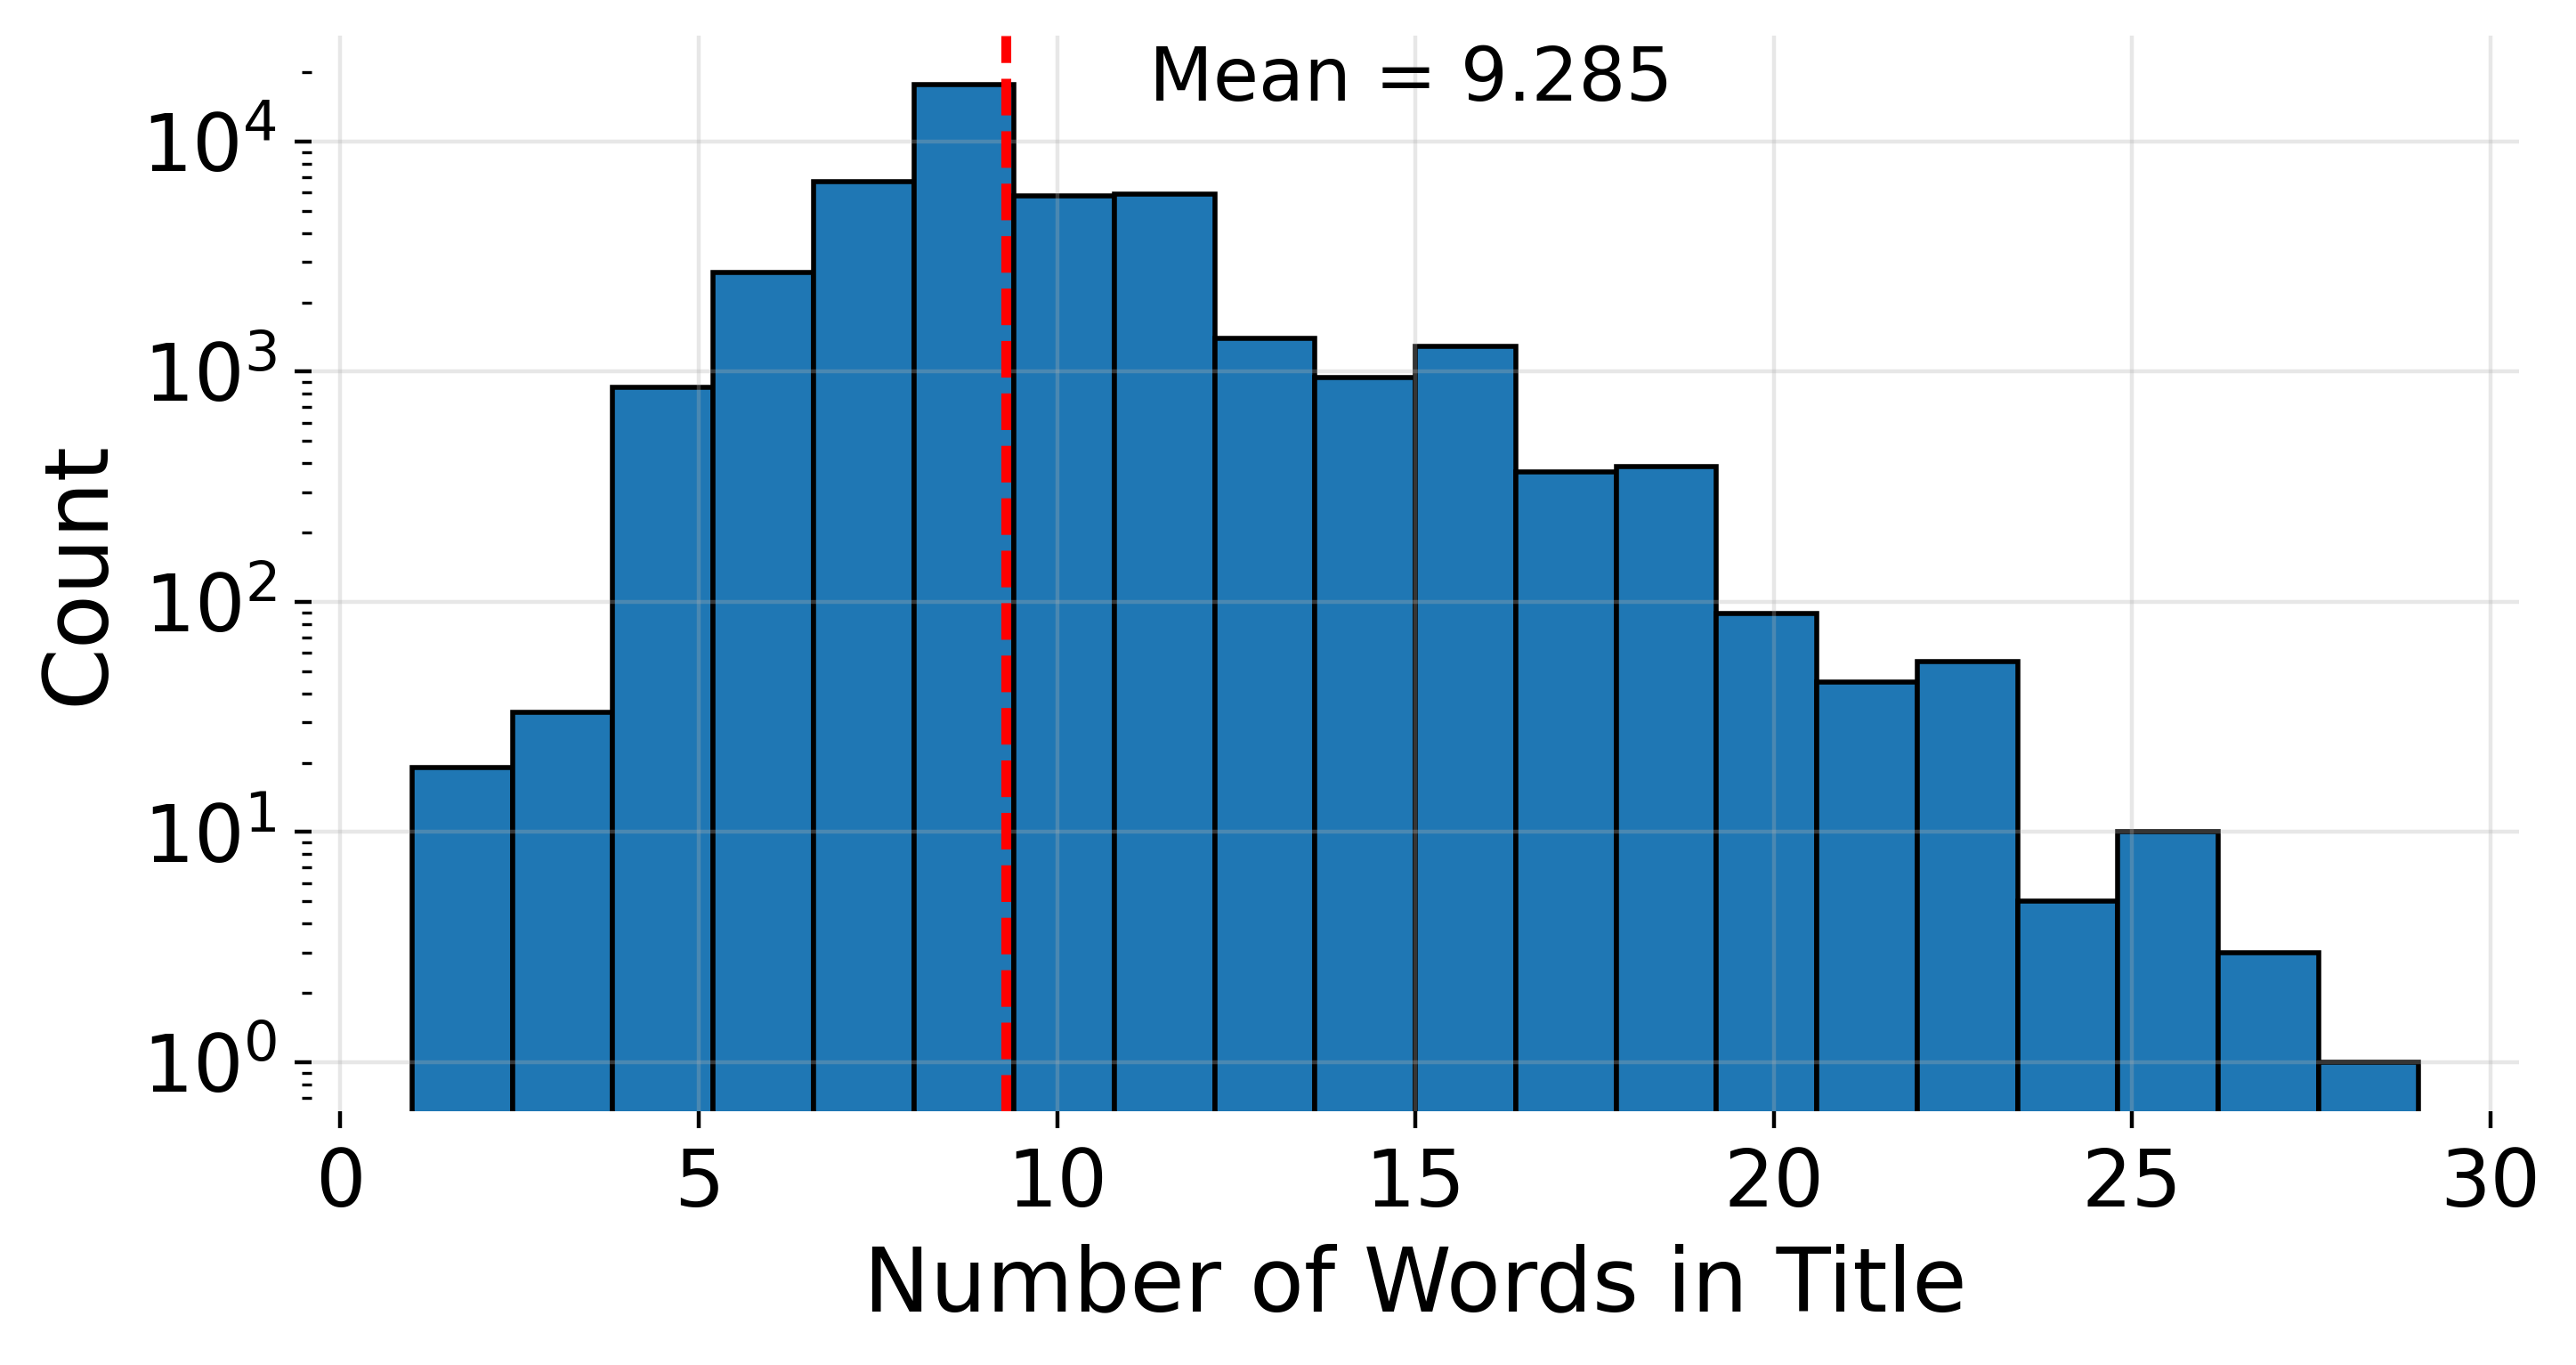
\includegraphics[scale=1]{../results/length_of_description.png}}
        \caption{Histogram of length of article titles. Mean description shown with verticle red line.}
        \label{fig:1}
\end{figure}	
	
	\section{Methods}
	
    Prior to training our classifiers, we first preprocessed the titles of the articles before vectorizing them to create our feature set. The preprocessing follows most of the standard steps used in other works\cite{oshikawa:2020}. We first extracted all of the titles from the dataframe for fake and true news. Then, we removed non-UTF-8 enocdable characters, removed punctuation from the titles using regular expressions, filtered out stopwords (e.g., ``at,'' ``and,'' ``the,'') using the list of english stopwords in the NLTK python library, and stemmed the text using the Porter stemming algorithm in NLTK. Text preprocessing is a staple for most NLP tasks because it removes language artifacts and casts the words into a more general form. In the case of this works, the text preprocessing reduces the dimensionality of the final feature space once we vectorize it by removing words and converting a number of different forms of the same word to a common stem. The preprocessed article titles are cast to numerical representations by turning them to one-hot vectors. The size of the vector is equal to the total number of unique words across all titles in the corpus. Each index corresponds to a single word. To vectorize a title, the feature vector gets a value of 1 if the word is present at all in that title (no matter how many times) and a 0 if it is not. This vectorization is done using the \texttt{feature\_extraction.text.CountVectorizer(binary = True)} function in sklearn. 
	
	The baseline models used in this work are all implemented in sklearn. The baseline models are described in Table \ref{table:2}. For this work, we chose some of the most widely used classifiers in the sklearn library. We implemented two support vector machine classifiers, one using a linear kernel and one using the radial basis function, logistic regression, multilayer perceptron, and naive bayes as our baselines. All classifiers use the default parameters used by sklearn. In this way our baseline models are not optimized classifiers with finely tuned hyperparameters. 
	
	We used the sklearn implementation of KNN as it is more computationally efficient than what we could implement. For PW, we created a simple implementation (see \texttt{parzen.py}). Our implementation of PW follows the algorithm outlined in class. To evaluate these nonparametric methods, we wanted to test a wide variety of hyperparameters. For KNN, tested with $k=$ 3, 5, 7, 9, 11, 13, 15, 17, 19, and 21, and for PW, we tested $h =$ 0.01, 0.05, 0.1, 0.5, 1, 5, 10, and 50.
	
	For the PW algorithm, we used an adjusted Gaussian kernel. Since the dimensionality of the feature space is $>18,000$, using a traditional multivariate Gaussian is problematic. We instead utilize the kernel outlined in Algorithm \ref{alg:1}.
	
	\begin{algorithm}
    \SetAlgoLined
    \KwData{$\frac{x - x_i}{h}$}
     Calculate $\tilde{x} = \sum_{j = 1}^{d} \frac{x - x_i}{h}$
     
     Initialize a 1D Gaussian distribution $g(y) \sim N(0,1)$
     
     \KwResult{$g(\tilde{x})$}
     \caption{Kernel function used for Parzen Window}
     \label{alg:1}
     \end{algorithm}
	
    For evaluation metrics, we report the accuracy score, area under the precision recall curve (auPRC), area under the receiver operator curve (auROC), F1 score (F1) and the computation time. We chose to report all of these metrics because each details a difference aspect of the classifiers. The computation time is a combination of the training and testing phases. Accuracy and auROC give a broad description of the classifier and are the most widely used classifier metrics, but they are insensitive metrics when class imbalances are present. As noted, the imblanace here is comparatively minimal, but we want to include metrics which are more sensitive to imbalances. Therefore, we also include auPRC and F1, which take into account both precision and recall. Computation time is reported to give an idea of the cost associated with using these classifiers. Reported metrics are averaged over 5-fold cross validation. Class balance is maintained across 5-fold cross validation to ensure representative training. 
		
	

	\section{Results}
	
    The results for our baselines are shown in Table \ref{table:2}. The KNN and PW results are shown in Table \ref{table:3} and \ref{table:4}, respectively. A plot showing performance versus computation time is shown in Figure \ref{fig:2}.
    
    %% Baselines
    \begin{table}[]
    \centering
    \begin{tabular}{|c|c|c|c|c|c|}
    \hline
    \textbf{Method} & \textbf{Accuracy} & \textbf{auPRC} & \textbf{F1} &                             \textbf{auROC} & \textbf{Time} \\ \hline
    \textbf{Linear SVM} & 0.95 & 0.92 & 0.95 & 0.95 & 19752.63 \\ \hline
    \textbf{Log Reg}    & 0.95 & 0.92 & 0.95 & 0.95 & 126.59   \\ \hline
    \textbf{MLP}        & 0.94 & 0.90 & 0.93 & 0.94 & 1506.45  \\ \hline
    \textbf{NB}         & 0.80 & 0.71 & 0.82 & 0.80 & 21.52    \\ \hline
    \textbf{RBF SVM}    & 0.95 & 0.93 & 0.95 & 0.95 & 25225.82 \\ \hline
    \end{tabular}
    \caption{Baseline model results averaged over 5-fold cross validation. Times shown are in seconds. Linear SVM: sklearn implementation of support vector classifier (SVC) with default parameters using a linear kernel. Log Reg: sklearn implementation with default parameters. MLP: sklearn implementation of multilayer perceptron with default parameters. NB: sklearn implementation of naive bayes classifier with default parameters. RBF SVM: sklearn implementation of SVC with default parameters using radial basis function as the kernel.}
    \label{table:2}
    \end{table} 
    
    
    %% KNN
    \begin{table}[]
    \centering
\begin{tabular}{|c|c|c|c|c|c|}
\hline
\textbf{Method} & \textbf{Accuracy} & \textbf{auPRC} & \textbf{F1} & \textbf{auROC} & \textbf{Time} \\ \hline
\textbf{3}  & 0.77 & 0.71 & 0.74 & 0.77 & 11176.50 \\ \hline
\textbf{5}  & 0.74 & 0.69 & 0.69 & 0.74 & 10014.54 \\ \hline
\textbf{7}  & 0.72 & 0.67 & 0.64 & 0.71 & 11483.15 \\ \hline
\textbf{9}  & 0.70 & 0.65 & 0.60 & 0.69 & 11389.89 \\ \hline
\textbf{15} & 0.68 & 0.64 & 0.55 & 0.67 & 10377.58 \\ \hline
\textbf{17} & 0.69 & 0.65 & 0.57 & 0.68 & 10979.94 \\ \hline
\textbf{19} & 0.70 & 0.66 & 0.58 & 0.69 & 10967.81 \\ \hline
\textbf{21} & 0.71 & 0.66 & 0.60 & 0.70 & 11090.60 \\ \hline
\end{tabular}
\caption{KNN results averaged over 5-fold CV. Times shown are in seconds.}
\label{table:3}
\end{table}
    
    %% Parzen Window
    \begin{table}[]
    \centering
\begin{tabular}{|l|l|l|l|l|l|}
\hline
              & \textbf{Accuracy} & \textbf{auPRC} & \textbf{F1} & \textbf{auROC} & \textbf{Time} \\ \hline
\textbf{0.01} & 0.74              & 0.65           & 0.76        & 0.74           & 50233.05      \\ \hline
\textbf{0.05} & 0.74              & 0.65           & 0.76        & 0.74           & 49052.06      \\ \hline
\textbf{0.1}  & 0.74              & 0.65           & 0.76        & 0.74           & 67516.09      \\ \hline
\textbf{0.5}  & 0.74              & 0.65           & 0.76        & 0.74           & 68830.92      \\ \hline
\textbf{1}    & 0.73              & 0.65           & 0.76        & 0.74           & 48808.16      \\ \hline
\textbf{5}    & 0.69              & 0.61           & 0.75        & 0.70           & 57335.28      \\ \hline
\textbf{10}   & 0.69              & 0.61           & 0.75        & 0.70           & 68715.34      \\ \hline
\textbf{50}   & 0.69              & 0.61           & 0.75        & 0.70           & 50593.84      \\ \hline
\end{tabular}
\caption{Parzen window results averaged over 5-fold CV. Times shown are in seconds.}
\label{table:4}
\end{table}
    
    %% Accuracy vs. Time
    \begin{figure}[htbp]
        \centerline{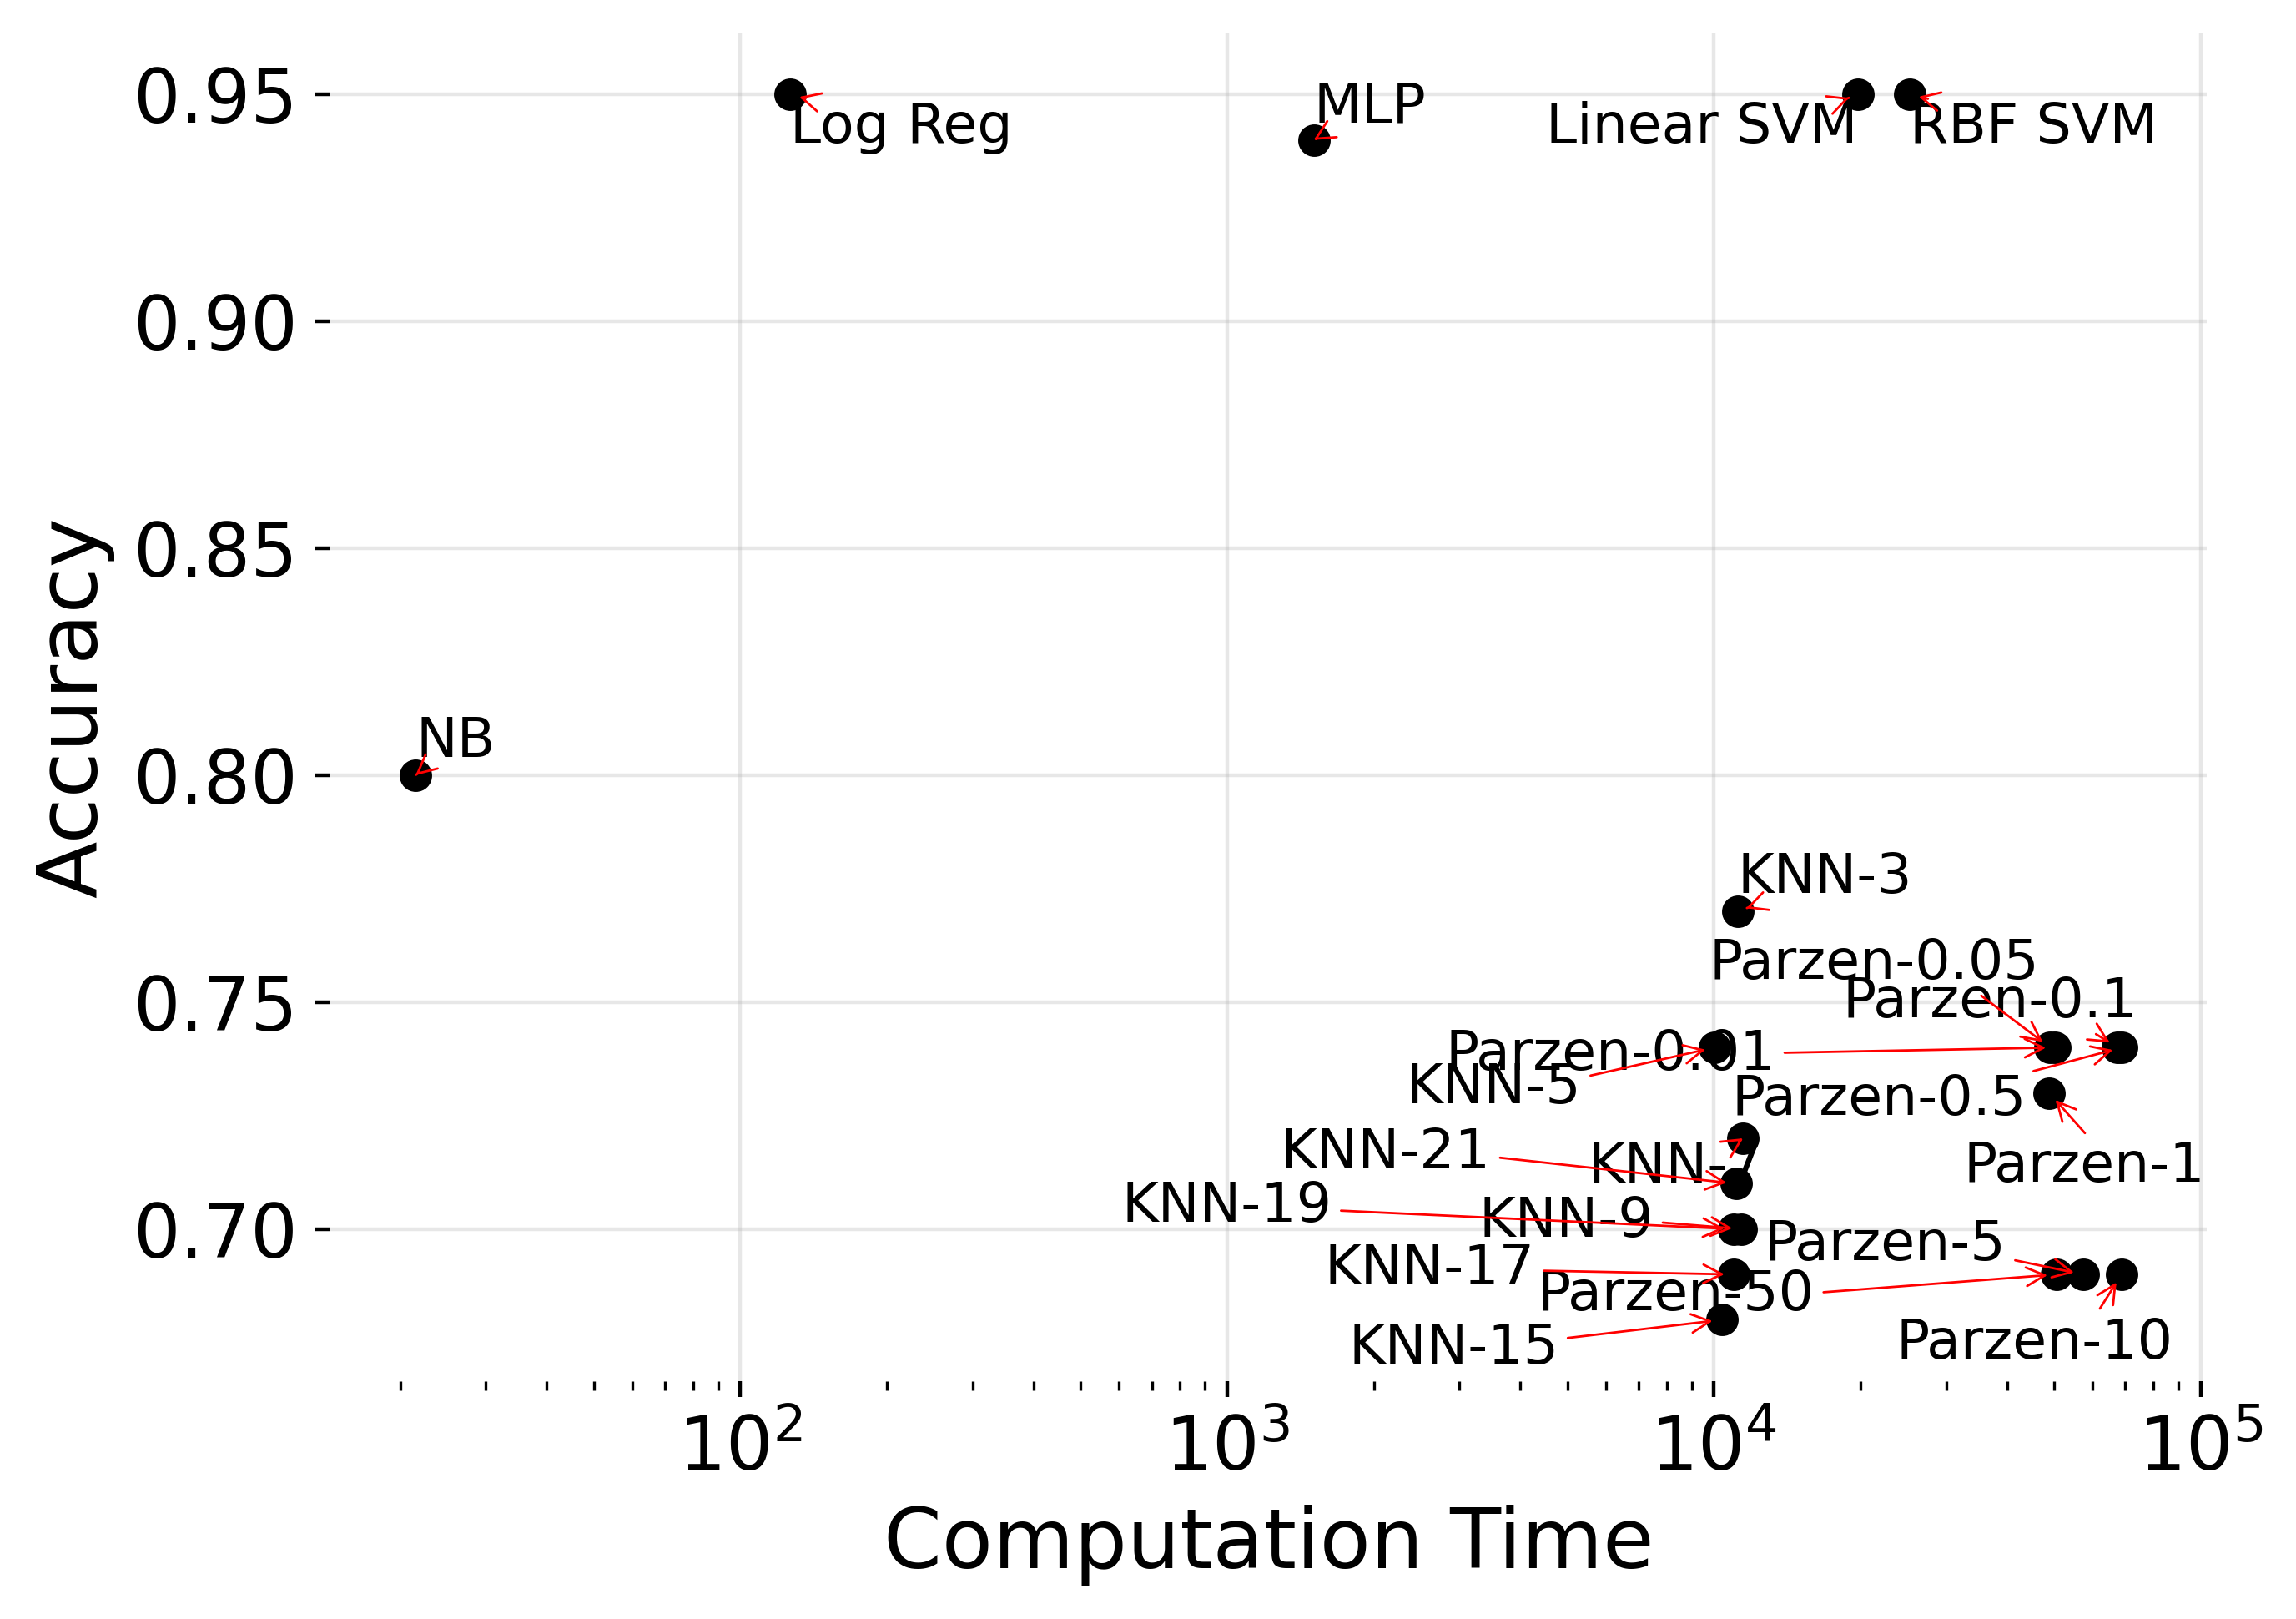
\includegraphics[scale=1]{../results/accuracy_vs_computation.png}}
        \caption{Plot of average accuracy from cross validation versus average computation time from cross validation. Points are labeled by their associated model. Arrows indicate connections between labels and points in congested areas of the plot.}
        \label{fig:2}
    \end{figure}
	
	\section{Discussion and Conclusions}
	
	We note that both nonparametric classification methods perform poorly on this classification task using this dataset. KNN achieved a maximum accuracy of 0.77 ($k = 3$) and a maximum auROC of 0.77 ($k=3$). However, if we examine the baseline results (Table \ref{table:2}), we see that the best performing KNN model doesn't outperform the worst baseline model (Naive Bayes, accuracy of 0.80 and auROC of 0.80). A similar result can be seen with PW, where the best performing models ($h = 0.01, 0.05, 0.1, 0.5$) do not match the performance of the worst baseline. As a general note, we do see KNN outperform PW on this task using this dataset. The best performing models that we tested are logistic regression and SVM with a linear kernel, both of which achieved an accuracy of 0.95 and an auROC of 0.95.
	
	In our tests, the nonparametric methods were unable to outperform the baseline models. There could be a number of possible reasons behind this failure. No feature selection was done with these features. Since each index in our feature space encodes for a specific ``word'' (stem after preprocessing), by reducing the dimensionality, we lose that information. However, by choosing to keep the full dimensionality of the problem, we incur large computation times and perhaps a loss of accuracy on these distance based methods such as KNN and PW. We also did not experiment with other kernels for PW. The kernel is a fundamental hyperparameter that ultimately determines the classifiers behavior. An area of future work could be to experiment with additional kernel functions. This could not only improve PW performance to meet or exceed the baseline models, but could also shed light onto the aspects of this dataset that are important to consider when making these classifications. Additionally, a different set of representative features could be used for these texts. We used a one-hot encoding for the article titles. These feature vectors are exceedingly spare with on average 9 out of 18,000 features being nonzero. We could have instead used representations determined by deep learning models like word2vec or BERT, which are trained on very large text corpora and cast text to dense numerical representations that capture language semantics. These denser representations may improve performance further by giving distance-based methods like KNN and PW more information to work with. They often times are of lower dimension as well (e.g., 1024), so computation times may be improved. Additional text from the article body itself, rather than the title alone, could be included in the prediction task to further provide models with a richer source of information to use for making predictions.
	
	A striking result of this work is shown in Figure \ref{fig:2}. This plot compares computational time with achieved accuracy. Ideally, we want to choose points in the upper left of the plot. These represent methods which are very fast to use and achieve a high accuracy. Based on these criteria, the most optimal choice of model for this classification task using this dataset is logistic regression as it is implemented by default in sklearn. Not only is it one of the most accurate of the models we evaluated, but it is orders of magnitude faster than most of the other methods we tested. In particular, we see that all of the nonparametrics methods are in the lower right hand side of the plot, which represent poorly performing models that require a large amount of computation time. PW and KNN are very costly to implement in this case because of the dimensionality of our problem. With over 40,000 samples each with more than 18,000 features, calculating pairwise information becomes exceedingly expensive. Additionally, without further feature engineering, the sparsity of these features may pose additional hinderances to these models. It should be noted that computation time is an issue across the board. With the exception of logistic regression, naive bayes, and the multilayer perceptron, computation times were on the order of hours, and in some cases 10s of hours. From a practical standpoint, these methods are not widely usable based solely on that point. In particular, our unoptimized implementation of PW is exceedingly slow compared to the other methods. While further optimization of the code may improve its performance, we see that the sklearn implementation of KNN was still on the order of hours, which does not bode well for our other nonparametric classifier. However, it should be noted that optimization may improve that aspect of our results.
	
	This work provides a comprehensive benchmarking of two nonparametric classifiers, KNN and PW, on the task of predicting whether a news article is true or not using a one-hot representation of the title alone. We have shown that these nonparametric methods are unable to outperform a set of baseline models with default parameters from the sklearn python library. We have, on the other hand, shown that there exists a model (e.g., logistic regression, linear SVM, MLP) that can accurately ($\geq 0.94$) delineate between fake and true news using only the article title. We have also shown that this can be done incredibly fast compared to other classifiers by using logistic regression.
	
	\section{Code Availability}
	
	Our code is available at \href{https://github.com/nathawkins/cse802_ss2021}{this GitHub repository}.    
	    
    %% Bibliography
    \newpage
    \bibliography{report} 
    \bibliographystyle{ieeetr}
	
\end{document}
